\section{面向开放组织的迷你看板实现}
\par 本项目实现的是一个基于Chromium内核的浏览器插件,可支持一系列带有Chromium内核的单核或多核浏览器,如Edge、Chrome、360安全浏览器、360极速浏览器等。

\subsection{开发框架与语言}
% React + TypeScript
\par 浏览器扩展程序基于HTML、CSS与JavaScript等前端技术构建。为了提升开发效率与代码可维护性,选择基于React框架进行开发。React是一个开源的、声明式、高效且灵活的用于构建用户界面的JavaScript库,使用React可以方便的基于组件逻辑创建复杂的交互式UI。
\subsection{技术架构}
% 前后端结构
% Hypertrons-crx是一个工具(chrome插件的形式),你需要把这个工具的开发构建过程,说清楚,感觉论文里面还差很多
\begin{figure}[H]
    \centering
    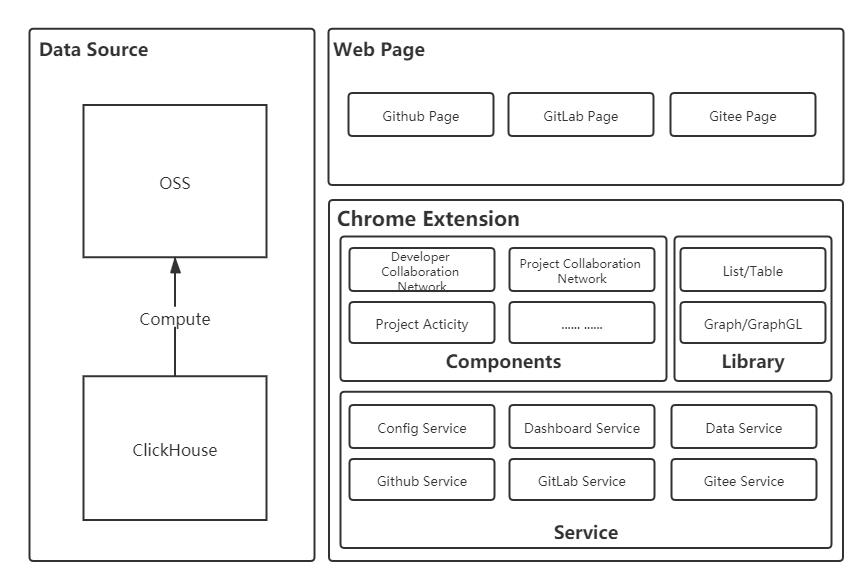
\includegraphics[width=150mm]{./figures/image5-1.png}
    \caption{技术架构图\\Technical architecture diagram}
\end{figure}
\par 面向开放社区的迷你看板的搭建过程本质上是一个浏览器插件的开发,从后端到前端,分为数据源、插件主体、前端页面三个部分。
\par 在数据源部分,后端由Hypertrons收集的开放平台全域数据存储在ClickHouse数据库中,按照上文所述的定义与计算方法,计算得到具体的字段数值,作为静态对象存储到OSS(Object Storage Service,阿里云对象存储)服务中,供前端直接调用。
\par 在插件主体部分,使用Typescript类定义各可视化图表组件,作为可以调用的模板,提供接口以嵌入真实的数据。同时,在该部分构建了配置服务、仪表盘服务,并联通后端的数据服务和3个开放平台(Github、GitLab和Gitee)的服务接口。其中,配置服务负责维护一个存储用户配置信息的json文件,每一次向后端发起请求、渲染图表之前,都去读取;仪表盘服务则负责取得数据、嵌入可视化组件模板,生成图表以插入到前端页面。
\par 在前端页面部分,则根据Github、GitLab、Gitee三个开放平台的UI风格,选择了与原生样式相近的组件库FrontUI,在原网页布局的基础上,将仪表盘服务生成的图表插入到页面的特定位置,如边栏、文本间等。

\par 在这个基础上,考虑到开发便利性与项目的国际化程度,在功能实现、架构搭建的基础上,还使用了chrome的i18n架构以增添插件对不同语言的支持,使用了静态代码分析工具ESLint、代码格式化工具Prettier和同为开源项目的工具Husky来使代码规范化。这些工作是为了保障本项目作为开源项目的开放性。



\subsection{高可配能力的实现}
\par 项目所有的配置都从代码仓库中的配置文件 .github/hypertrons.json 中读取,即:
插件所提供的功能由配置文件决定,配置文件配置在项目中,基于 Git 进行管理和迭代,公开透明。
同一项目下的所有安装该插件的用户,Perceptor 提供的是相同的能力。
同一用户,在不同项目页面下,看到的是不同的看板。


\subsection{数字化看板模块的实现}
% 各个功能对应的技术手段
\par 项目基于Echarts提供数据可视化图表渲染能力。Echarts是一个使用JavaScript实现的开源可视化库,提供直观、交互丰富、可高度个性化定制的数据可视化图表。通过对Echarts进行封装,并基于Hypertrons后端获取数字化看板的配置信息以及各个平台的开放数据,就可以根据每个社区/组织的自身业务场景,实现高度可配的数字化看板。基于此,能够实现支持每一位用户基于自身权限地配置浏览器页面的数字化看板\cite{deqingli2018echarts}。
\par 以GitHub项目数字化看板展示为例,可从hypertrons后端获取得到数字化看板的配置信息,以及项目的Repository、Issue、Pull request和从其他平台采集得到的开放数据,然后根据用户自定义的配置信息生成相应的可视化组件,再经由浏览器插件,以HTML的格式注入到用户浏览的当前页面,完成整个呈现\cite{陈挺2016ng}。



\subsection{跨平台交互模块的实现}
\par 在浏览器页面中输入的交互式命令行会由浏览器插件传递到hypertrons 后端,由hypertrons 后端运行、完成指定操作后后,再通过浏览器插件,反馈结果给来自不同平台、使用不同语言的用户,从而提供跨平台交互的能力。

\subsection{跨平台实时消息通知与配置管理模块的实现}
\par 跨平台实时消息通知与配置管理模块是基于浏览器插件的特性,在Chromium提供的用于浏览器插件开发的官方接口上进行实现。其本质是前后端之间信息的简单传递。

\subsection{身份认证与权限管理模块的实现}
\par 用户能够在开源平台的设置项中管理自己的Token,而当用户为迷你看板插件配置了个人账户的Token,即迷你看板插件获得了该用户账号的部分权限。获得用户Token之后,插件将读取的用户名和头像自动显示,并且该Token会在后续发生的一系列请求访问中自动使用。

\subsection{功能测试}
% Jest
\par 项目使用Jest,一个简洁的测试框架,它能够很好地与Typescript以及React框架共用。Jest在大部分基于JavaScript的项目上可以实现开箱即用、无需配置,且具有优秀的 api,易于书写与维护。
% //TODO: 测试了哪些功能点


% //TODO: 最后要不要放效果图?-先不放上去,准备着
% \subsection{实现结果}
% 项目、个人Github主页最终效果(贴图)


